\chapter{Methodology}
\label{chap:method}

% Outline approved 2 November 2026 (notes/chapter3-outline.md). The design is
% fixed in notes/method-design.md; code/ implements it. Sources for every
% claim are listed in notes/chapter3-claims.md.
%
% Conventions while data collection is pending:
%  - \TBC{...}  (red, in brackets): a value set during data collection, e.g.
%    the band, the gain settings or the number of sessions captured.
%  - \Prov{...} (red): a provisional starting setting that may still be tuned
%    on training and validation data; frozen before the test data are scored.
%  - The chapter is written in the present tense as a description of the
%    design. Once the captures exist and the code has been run, it is to be
%    converted to the past tense with the values actually used.

\section{Introduction}
\label{sec:m-intro}

This chapter describes how the research questions of Chapter~1 are answered. It sets out the research design (\cref{sec:m-design}), the receiver, the band survey and the capture settings (\cref{sec:m-hardware}), the data classes and the capture sessions (\cref{sec:m-data}), the ground truth (\cref{sec:m-labels}) and the controlled-SNR test set (\cref{sec:m-injection}). It then describes the preprocessing (\cref{sec:m-preproc}), the session-level data splits (\cref{sec:m-splits}), the detectors (\cref{sec:m-detectors}) and the calibration of their thresholds (\cref{sec:m-thresholds}). The evaluation protocol, including the tests of the two hypotheses, is given in \cref{sec:m-eval}, the measurement of computational cost in \cref{sec:m-compute} and the real-time demonstration in \cref{sec:m-demo}. \Cref{sec:m-ethics} covers ethics, reproducibility and threats to validity, and \cref{sec:m-summary} summarizes the chapter.

\section{Research Design}
\label{sec:m-design}

The study is a comparative, quantitative evaluation of detectors on real captures. Every detector receives exactly the same frames of complex baseband samples recorded with the RTL-SDR Blog V4, and every detector is operated at the same false-alarm probabilities, calibrated in the same way on idle data that none of them has been trained on. Two kinds of test data are used. The over-the-air captures themselves are the uncontrolled conditions: their signal-to-noise ratio (SNR) and noise floor vary naturally between sessions, days and positions. A controlled-SNR test set, built by adding scaled LTE captures to idle captures in software, provides exact labels at set SNRs (\cref{sec:m-injection}). Data are split by capture session, never by frame, and every session is used as test data exactly once through session-level cross-validation (\cref{sec:m-splits}). Uncertainty is estimated over training seeds and, by bootstrap resampling, over sessions (\cref{sec:m-eval}).

\Cref{fig:m-overview} shows the pipeline from capture to evaluation, and \cref{tab:m-rq-map} links each research question and hypothesis to the data, detectors and analyses that address it.

\begin{figure}[tbp]
  \centering
  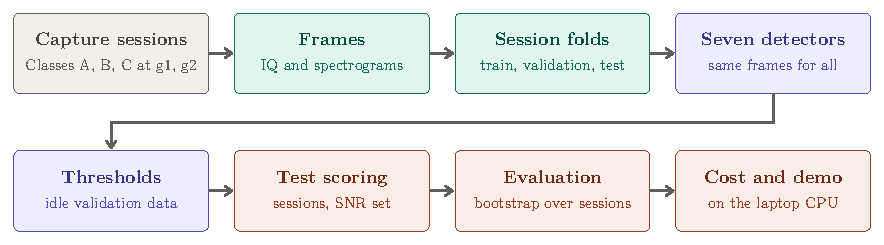
\includegraphics[width=\textwidth]{fig3-overview}
  \caption[Overview of the method]{Overview of the method. Captures from each session are framed and preprocessed once; all detectors score the same frames; thresholds are calibrated on idle validation sessions; test sessions and the controlled-SNR set are scored and evaluated with session-level uncertainty.}
  \label{fig:m-overview}
\end{figure}

\begin{table}[tbp]
  \centering
  \small
  \caption[Research questions and hypotheses mapped to the analyses]{Research questions and hypotheses of Chapter~1 mapped to the data, detectors and analyses of this chapter.}
  \label{tab:m-rq-map}
  \begin{tabularx}{\textwidth}{@{} >{\raggedright\arraybackslash}p{1.3cm} >{\raggedright\arraybackslash}X >{\raggedright\arraybackslash}X >{\raggedright\arraybackslash}X @{}}
    \toprule
    Item & Data & Detectors & Analysis \\
    \midrule
    RQ1 & Test sessions; controlled-SNR set & Convolutional autoencoder; fixed and adaptive energy detectors & $\Pd$ at $\Pfa = \pct{1}$ and \pct{5} by SNR (\cref{sec:m-eval}) \\
    RQ2 & As RQ1 & Convolutional autoencoder; PCA; \syncsignal{} correlator & As RQ1; paired differences with session bootstrap \\
    RQ3 & Pooled test folds; gain-$g_2$ captures & All & Realized $\Pfa$ and $\Pd$ across sessions, days, positions and the gain change \\
    RQ4 & Laptop CPU & All & Latency, throughput, real-time factor (\cref{sec:m-compute}) \\
    RQ5 & As RQ1 & Convolutional and fully connected autoencoders; VAE with MSE and percentile scores & As RQ1, with latent-size ablations \\
    H1 & Controlled-SNR set, SNR $\le \qty{-4}{\decibel}$ & Convolutional autoencoder versus adaptive energy detector & Bootstrap interval of $\Delta\Pd$ (\cref{sec:m-hypotheses}) \\
    H2 & Gain-$g_2$ captures of the test sessions & Convolutional autoencoder versus fixed energy detector (adaptive as reference) & Departures of realized $\Pfa$ and $\Pd$ from calibrated values (\cref{sec:m-hypotheses}) \\
    \bottomrule
  \end{tabularx}
\end{table}

\section{Hardware, Software and Band Selection}
\label{sec:m-hardware}

\subsection{Receiver and Host Computer}
\label{sec:m-receiver}

All captures are made with a single RTL-SDR Blog V4, whose specifications were summarized in \cref{tab:rtlsdr-v4}. It has an R828D tuner and an RTL2832U converter with 8-bit samples, tunes from \qty{500}{\kilo\hertz} to \qty{1.766}{\giga\hertz}, has a stable bandwidth of about \qty{2.56}{\mega\hertz} and a temperature-compensated reference oscillator with a tolerance of \qty{1}{ppm}, and provides a bias tee that can be switched in software \parencite{rtlsdrblog2024}. The receiver is connected over USB to the host laptop, a Dell Latitude 5490 with an Intel Core i5-8250U processor (four cores, eight threads), \qty{16}{\giga\byte} of memory and integrated graphics, running Ubuntu 26.04. All processing runs on the laptop's CPU except the training of the neural networks, which runs on a cloud graphics processing unit (GPU) provided by Google Colab (\cref{sec:m-training}). The trained detectors are scored, timed and demonstrated on the laptop, which is where a detector of this kind would be used. The software is written in Python and uses PyTorch \parencite{paszke2019} for the neural networks and scikit-learn \parencite{pedregosa2011} for PCA. \Cref{tab:m-hw-sw} lists the hardware and software, and \cref{app:install} describes how the receiver driver, the Python environment and the cell-search tool are installed.

\begin{table}[tbp]
  \centering
  \caption[Hardware and software]{Hardware and software used in the study. Library versions are those pinned in the project's lock file (\texttt{code/uv.lock}).}
  \label{tab:m-hw-sw}
  \begin{tabularx}{\textwidth}{@{} l >{\raggedright\arraybackslash}X @{}}
    \toprule
    Item & Value \\
    \midrule
    Receiver & RTL-SDR Blog V4 (R828D, RTL2832U, 8 bits) \\
    Antenna & \TBC{model, recorded in the capture metadata} \\
    Host & Dell Latitude 5490, Intel Core i5-8250U, \qty{16}{\giga\byte} RAM \\
    Operating system & Ubuntu 26.04 LTS \\
    Python & 3.12 \\
    PyTorch (CPU build) & 2.12.0 \\
    NumPy, SciPy & 2.4.5, 1.18.1 \\
    scikit-learn & 1.9.1 \\
    pyrtlsdr & 0.2.91 \\
    Receiver driver & \texttt{rtl-sdr-blog}, the manufacturer's fork of the RTL-SDR library, commit aed0ea1, built from source \parencite{rtlsdrblog2026} \\
    Survey tool & \texttt{rtl\_power} (from the RTL-SDR driver package) \\
    Cell-search tool & LTE-Cell-Scanner, program \texttt{CellSearch}, commit e7f71cb \parencite{peroulas2024} \\
    Training hardware & Google Colab GPU (\TBC{type and library versions, as recorded}) \\
    \bottomrule
  \end{tabularx}
\end{table}

\subsection{Band Survey}
\label{sec:m-survey}

Before any data are captured, the candidate bands are surveyed at the capture site. The survey's own measurements are not used to train or test any detector. Its role is to decide where and how the receiver is tuned for every capture that is used, and to document those decisions. Five settings of the study depend on it (\cref{tab:m-survey-role}).

\begin{table}[tbp]
  \centering
  \small
  \caption[Settings decided by the band survey]{Settings decided by the band survey.}
  \label{tab:m-survey-role}
  \begin{tabularx}{\textwidth}{@{} >{\raggedright\arraybackslash}p{3.0cm} >{\raggedright\arraybackslash}X >{\raggedright\arraybackslash}X @{}}
    \toprule
    Setting & Found from & Why it matters \\
    \midrule
    Band studied & Plateaus confirmed as carriers by the cell search, in every candidate range & An allocation does not mean that a carrier is on air at the site \\
    Carrier centre and bandwidth & Cell search on the chosen plateau & They place the C\textsubscript{centre} and C\textsubscript{offset} windows; C\textsubscript{offset} needs a carrier of at least \qty{10}{\mega\hertz} \\
    Idle (Class~B) window & A stretch of at least \qty{1.92}{\mega\hertz} with no signal above the noise floor, outside every carrier found & Its captures train the reconstruction models and give the idle frames of every evaluation \\
    Gains $g_1$ and $g_2$ & The strongest carrier, with trial captures & The strongest active capture must not clip the 8-bit converter \\
    Stability over the day & Surveys by day and at night & The carrier must be on air, and the idle window empty, at both session times \\
    \bottomrule
  \end{tabularx}
\end{table}

\emph{Sweeps.} Each candidate range is swept with \texttt{rtl\_power}, the spectrum-survey program of the RTL-SDR driver, at a fixed gain of \qty{40.2}{\decibel}, one of the tuner's steps; automatic gain is not used, for the same reason as in the captures (\cref{sec:m-capture}). The program steps the receiver across the range and records the power in frequency bins at most \qty{25}{\kilo\hertz} wide, averaged over \qty{10}{\second}. Each range is swept for \qty{10}{\minute}, which gives 60 readings for every bin. The readings are plotted as the mean power against frequency, together with the maximum over the readings, and as a waterfall of power against frequency and time. A narrow spike appears at the centre frequency of every tuning step of the sweep, in every reading; it is produced by the receiver, not by a signal, and is ignored. The sweep lasts minutes rather than seconds so that steady and intermittent signals can be told apart. A cell transmits reference signals in every downlink subframe \parencite[clause~6.10.1]{3gpp2026a}, so an active LTE carrier raises the power in every reading and appears as a flat plateau whose width matches one of the channel bandwidths of \cref{tab:lte-bandwidths}. An intermittent signal raises it in only some readings: it shows in the maximum but hardly in the mean, and as isolated marks in the waterfall. A single short sweep could not distinguish the two.

\emph{Cell search: why.} A plateau shows only that power is present in part of a range. It does not show which system transmits it, and its edges, blurred by the coarse bins of the sweep, give only estimates of where the signal begins and ends. A cell search settles both questions, and four parts of the method depend on it:
\begin{itemize}
  \item \emph{It confirms that a plateau is an LTE carrier.} The search detects the primary and secondary synchronization signals defined by the LTE standard \parencite[clause~6.11]{3gpp2026a} (\cref{sec:lte-sync}). A plateau counts as a carrier only if a cell is found at its centre, and the band studied is chosen among confirmed carriers only.
  \item \emph{It gives the carrier's exact centre and bandwidth.} The C\textsubscript{centre} window must be centred on the carrier, where the synchronization signals are, and the C\textsubscript{offset} window is placed at a distance from the centre that depends on the occupied width (\cref{sec:m-classes}). Both need the centre and bandwidth reported by the search, not estimates from the survey.
  \item \emph{It supports the ground truth.} A Class~C capture is labelled occupied only once a cell search has confirmed an active cell on the carrier (\cref{sec:m-labels}), and the cell identity shows whether the same cell is received in every session.
  \item \emph{It checks the idle window.} The centre and bandwidth of each carrier near the idle window show whether the window lies outside the band that the carrier occupies.
\end{itemize}

\emph{Cell search: how.} The search uses \texttt{CellSearch}, the cell-search program of LTE-Cell-Scanner, which was written for RTL2832-based receivers and is built here for the RTL-SDR \parencite{peroulas2024}. It tunes the receiver, at a fixed gain, to each frequency of a range in steps of \qty{100}{\kilo\hertz}, looks for the primary and secondary synchronization signals of a cell, and decodes the master information block (MIB) that the cell broadcasts. For each cell found it reports the physical-layer cell identity, the carrier frequency, the frequency offset, the received power and the bandwidth in resource blocks \parencite{peroulas2024}, which gives the carrier's channel bandwidth (\cref{tab:lte-bandwidths}). After each survey run, every plateau whose width is close to the occupied width of an LTE channel bandwidth is searched from \qty{0.5}{\mega\hertz} below to \qty{0.5}{\mega\hertz} above its centre, rounded to \qty{0.1}{\mega\hertz}, at a gain of \qty{40.2}{\decibel} and with two tries at each frequency. The program's output is kept with the survey records (\cref{app:survey}). At every session the search is repeated at the chosen carrier's frequency alone, before the captures, and the samples it captured are kept; the cell identity must be the one found in the survey.

\emph{Band.} The band cannot be fixed in advance. The candidate downlink ranges are those of \cref{tab:lte-bands} that the receiver can tune: \qtyrange{758}{803}{\mega\hertz} (Band~28), \qtyrange{790}{894}{\mega\hertz} (Bands~20 and~5 together) and \qtyrange{925}{960}{\mega\hertz} (Band~8). An allocation only permits operators to use a band; it does not show whether, or where in the band, a carrier is on air in Benin City. The band studied is therefore the one with the best confirmed carrier at the site: \TargetBand. Within it, the \qty{10}{\mega\hertz} carrier centred at \qty{773}{\mega\hertz} (cell identity 145) is used for the active captures; the reasons for this choice are given in \cref{app:survey}. The survey outputs are kept as evidence for this and the other choices (\cref{app:survey}).

\emph{Windows.} The survey also fixes where the receiver's \qty{1.92}{\mega\hertz} window is placed (\cref{fig:m-windows}). For active captures (Class~C, \cref{sec:m-data}), it is placed either on the carrier's centre, where it contains the synchronization signals, or inside the carrier away from its centre, where it does not (\cref{sec:lte-sync}). For idle captures (Class~B), it is placed on a stretch of the surveyed range at least \qty{1.92}{\mega\hertz} wide with no carrier, as close as possible to the carrier, so that the idle and active captures are made at nearly the same tuner frequency. With the chosen carrier, the C\textsubscript{centre} window is centred at \qty{773}{\mega\hertz}, the C\textsubscript{offset} window \qty{2.52}{\mega\hertz} above it, at \qty{775.52}{\mega\hertz}, and the idle window at \qty{765.37}{\mega\hertz}, in a stretch that was quiet by night and by day (\cref{app:survey}).

Of all the settings, the idle window has the largest consequences. The reconstruction models learn whatever their training frames contain as normal (\cref{sec:ae-anomaly}), and their training frames are the Class~B captures at $g_1$ (\cref{sec:m-training}). The same captures give the idle frames on which every detector's threshold is calibrated and its false alarms are counted (\cref{sec:m-thresholds,sec:m-eval}). A weak signal in the idle window that went unnoticed would therefore be learned as part of the noise floor, so that the networks could not detect it, and it would make the idle label of every frame in the window wrong, in training and in evaluation alike. Because frames are not screened individually (\cref{sec:m-labels}), the window has to be shown to be empty before any idle data are captured. In every frequency bin of the window, the mean power must stay within \qty{3}{\decibel} and the maximum over the readings within \qty{6}{\decibel} of the noise floor, so that narrow and intermittent signals are excluded as well as carriers; and the window must lie outside the band occupied by every carrier that the cell search finds near it.

\emph{Gains and times.} The survey also shows the strongest carrier, at which trial captures are made to choose the gains $g_1$ and $g_2$ (\cref{sec:m-capture}). It is made once by day and once at night, starting at 07:00 and 22:00 WAT, the times of the sessions (\cref{sec:m-sessions}). Labels are set for whole captures (\cref{sec:m-labels}), so they hold only if the carrier is on air, and the idle window empty, at both times; a carrier that is off at one of the times, or a transmitter that appears in the idle window at one of them, shows as a difference between the two surveys. The survey is made at P1 (\cref{sec:m-sessions}), before the first session; each of its two runs takes about half an hour for the sweeps, followed by the cell searches. Before the first session at P2, the chosen carrier is searched for there and the range containing it is swept once for \qty{10}{\minute}, to confirm that the carrier is received and the idle window is quiet at P2 as well.

\begin{figure}[tbp]
  \centering
  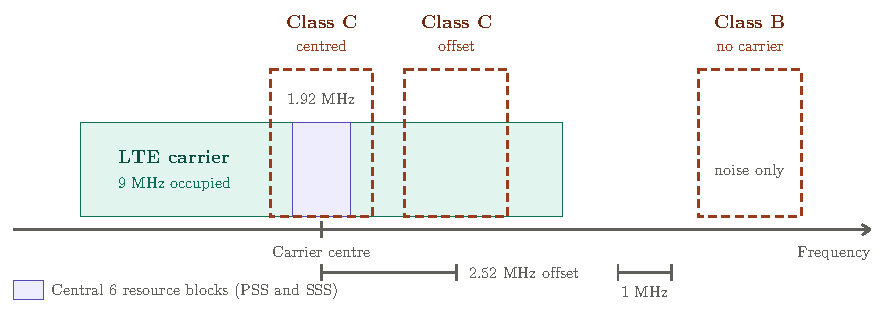
\includegraphics[width=\textwidth]{fig3-windows}
  \caption[Placement of the receiver windows]{Placement of the \qty{1.92}{\mega\hertz} receiver window for the three window types, shown for an example \qty{10}{\mega\hertz} carrier (\qty{9}{\mega\hertz} occupied), to scale in frequency. C\textsubscript{centre} is centred on the carrier and contains the PSS and SSS; C\textsubscript{offset} lies inside the carrier, clear of the central six resource blocks; B lies in a stretch with no carrier. Carrier widths from \textcite[Table~5.6-1]{3gpp2026b}; the central six resource blocks from \textcite[clause~6.11]{3gpp2026a}.}
  \label{fig:m-windows}
\end{figure}

\subsection{Capture Configuration}
\label{sec:m-capture}

\emph{Sample rate.} The receiver samples at $f_s = \qty{1.92}{MS/s}$. LTE timing is defined in units of $T_s = 1/(15000 \times 2048)$~s \parencite[clause~4]{3gpp2026a}, so $1/T_s = \qty{30.72}{\mega\hertz}$ and $f_s$ is exactly one sixteenth of it. At this rate the useful part of an OFDM symbol, $2048\,T_s$, is 128 samples, and the normal cyclic prefix of $160\,T_s$ or $144\,T_s$ is 10 or 9 samples \parencite[clause~6.12, Table~6.12-1]{3gpp2026a}. A 128-point fast Fourier transform (FFT) then has a bin spacing of \qty{15}{\kilo\hertz}, equal to the LTE subcarrier spacing \parencite[Table~6.2.3-1]{3gpp2026a}, and the PSS can be correlated against templates generated directly at the sample rate (\cref{sec:m-pss}). The observed window, \qty{1.92}{\mega\hertz} wide, is within the receiver's stable bandwidth of about \qty{2.56}{\mega\hertz} \parencite{rtlsdrblog2024} and contains the central \qty{1.08}{\mega\hertz} of a carrier when centred on it.

\emph{Gain.} Automatic gain control is never used, because it would change the noise floor during a capture. Two fixed gain settings are used: $g_1$, the primary setting, and $g_2$, used only for the gain-change test of \cref{sec:m-robustness}. For every capture the fraction of in-phase or quadrature samples at the extremes of the 8-bit range is recorded, and captures with more than \Prov{\pct{0.1}} clipped samples are flagged. The gains were chosen with trial captures on the chosen carrier after the survey (\cref{app:gains}). $g_1$ is the highest tuner gain step at which captures centred on the carrier stay below this limit even during traffic peaks, in which the carrier's power was seen to rise by several decibels; $g_2$ is the step \qty{10}{\decibel} lower. This gave $g_1 = \qty{29.7}{\decibel}$ and $g_2 = \qty{19.7}{\decibel}$. At these gains the idle level is set mainly by the receiver's own noise: lowering the gain from $g_1$ to $g_2$ lowered the idle level by about \qty{2}{\decibel}, while the carrier's level fell by about \qty{8}{\decibel} (\cref{app:gains}).

\emph{Other settings.} The bias tee is off for every capture: it must be off with the \qty{50}{\ohm} terminator of Class~A, and the antenna is passive. No frequency correction is applied (\qty{0}{ppm}), since the reference oscillator's tolerance is \qty{1}{ppm} \parencite{rtlsdrblog2024}; the value is recorded. Recording begins after the first \num{131072} samples (\qty{68}{\milli\second}) of the stream have been discarded. Each capture then lasts \Prov{\qty{30}{\second}}, giving \num{57600000} complex samples, which are stored as interleaved 8-bit unsigned integers (about \qty{115}{\mega\byte} per capture) with a metadata file.

\subsection{Metadata}
\label{sec:m-metadata}

A metadata record is written with every capture (\cref{tab:m-metadata}). It identifies the session, the position and the data class, records every receiver setting, and stores the cell-search result and the version of the capture software, so that every frame used in the evaluation can be traced to the conditions under which it was recorded.

\begin{table}[tbp]
  \centering
  \small
  \caption[Metadata recorded with each capture]{Metadata recorded with each capture.}
  \label{tab:m-metadata}
  \begin{tabularx}{\textwidth}{@{} >{\raggedright\arraybackslash}p{3.4cm} >{\raggedright\arraybackslash}X @{}}
    \toprule
    Group & Fields \\
    \midrule
    Identity & Capture, session and position identifiers; data class (A, B, C\textsubscript{centre}, C\textsubscript{offset}); start and end time (UTC) \\
    Receiver & Model and serial string; antenna; centre frequency; sample rate; gain; frequency correction; bias-tee state \\
    Measurements & Number of samples; clipping fraction; mean power; temperature, if available \\
    Ground truth & Cell-search tool and result (cell identity, carrier centre, bandwidth if known); operator notes \\
    Provenance & Version of the capture software (Git commit) \\
    \bottomrule
  \end{tabularx}
\end{table}

\section{Data Collection}
\label{sec:m-data}

\subsection{Data Classes}
\label{sec:m-classes}

Data are captured in three classes, the third in two window placements (\cref{fig:m-setup}).
\begin{itemize}
  \item \emph{Class A, receiver noise.} The antenna input is terminated with a matched \qty{50}{\ohm} load, so the capture contains only the receiver's own noise. Class~A is used to track the receiver noise floor across sessions and gain settings, and as a check of false alarms caused by the receiver alone. It is not used to train any detector.
  \item \emph{Class B, idle spectrum.} The antenna is connected and the window is placed where there is no LTE carrier (\cref{sec:m-survey}). Class~B contains the receiver noise together with whatever the environment contributes, and it is the normal class from which the reconstruction models learn and on which all thresholds are calibrated.
  \item \emph{Class C, LTE active.} The antenna is connected and the window lies on an active LTE carrier, either centred on it (C\textsubscript{centre}) or offset inside it (C\textsubscript{offset}). The offset places the window midway between the edge of the central six resource blocks, at \qty{\pm 0.54}{\mega\hertz}, and the edge of the occupied band: $f_\mathrm{off} = (\qty{0.54}{\mega\hertz} + W_\mathrm{occ}/2)/2$, where $W_\mathrm{occ}$ is the occupied width of \cref{tab:lte-bandwidths}. A window of \qty{1.92}{\mega\hertz} fits there only if the channel bandwidth is at least \qty{10}{\mega\hertz}; for a \qty{10}{\mega\hertz} carrier, $f_\mathrm{off} = \qty{2.52}{\mega\hertz}$. If the chosen carrier is narrower, C\textsubscript{offset} is not captured.
\end{itemize}

\begin{figure}[tbp]
  \centering
  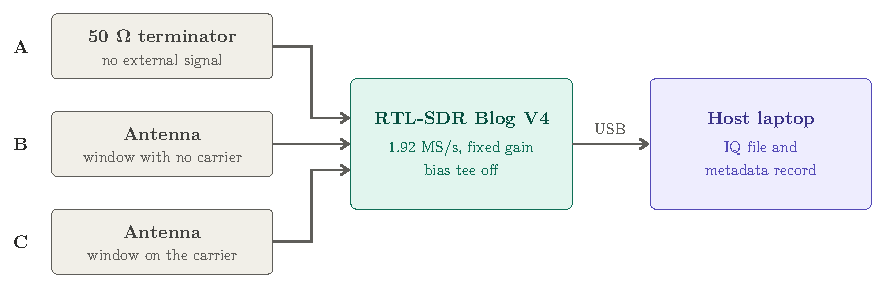
\includegraphics[width=\textwidth]{fig3-setup}
  \caption[Capture set-up for the data classes]{Capture set-up for the data classes. Class~A uses a \qty{50}{\ohm} terminator in place of the antenna; Classes~B and~C use the antenna and differ only in where the window is tuned (\cref{fig:m-windows}). The bias tee is off throughout.}
  \label{fig:m-setup}
\end{figure}

\subsection{Sessions}
\label{sec:m-sessions}

A session is one visit to one position, during which all classes are captured at both gain settings in a fixed order: A, B, C\textsubscript{centre} and C\textsubscript{offset}, each first at $g_1$ and then at $g_2$, so that the terminator is fitted and removed only once. That gives eight captures per session (\cref{tab:m-session-plan}). Sessions are the units of independence in the study: frames from the same session share the receiver's warm-up state, the antenna position and the local interference, so they are never split between training and test data. At least twelve sessions are planned, spread over at least four days and over two positions at the author's home in Benin City: the balcony of the sitting room (P1) and the balcony of a bedroom (P2). The two balconies face different directions, so the signals reach them from different directions and through different surroundings. At each position the antenna is mounted at a marked spot, at the same height and orientation in every session and at least \qty{30}{\centi\metre} from metal railings and bars, and the setup is photographed; the laptop stays indoors. Day sessions start at 07:00 and night sessions at 22:00 West Africa Time (WAT, UTC+1), the times of the survey. Each session is labelled day or night from the start time of its first capture; a session that starts more than two hours from both times is labelled off schedule and reported separately. The sessions actually captured are listed in \cref{app:sessions}.

\begin{table}[tbp]
  \centering
  \caption[Capture plan for one session]{Capture plan for one session. At \qty{1.92}{MS/s}, a \Prov{\qty{30}{\second}} capture yields \num{3515} frames of \num{16384} samples (\cref{sec:m-preproc}).}
  \label{tab:m-session-plan}
  \begin{tabular}{@{} c l l c c @{}}
    \toprule
    Order & Class & Window & Gain & Frames \\
    \midrule
    1, 2 & A & Antenna input terminated & $g_1$, $g_2$ & \num{3515} each \\
    3, 4 & B & No carrier & $g_1$, $g_2$ & \num{3515} each \\
    5, 6 & C\textsubscript{centre} & Carrier centre & $g_1$, $g_2$ & \num{3515} each \\
    7, 8 & C\textsubscript{offset} & Inside the carrier, off-centre & $g_1$, $g_2$ & \num{3515} each \\
    \bottomrule
  \end{tabular}
\end{table}

\section{Ground Truth}
\label{sec:m-labels}

Labels are set for whole captures, from the protocol and the cell search made at the time of capture. A Class~C capture is labelled occupied in every frame once the cell search has confirmed an active cell on the carrier. This is justified by the downlink structure: a cell transmits cell-specific reference signals in every downlink subframe \parencite[clause~6.10.1]{3gpp2026a}, so an active carrier occupies every frame of the window (\cref{sec:lte-sync}). A Class~B capture is labelled idle in every frame if the survey shows no signal in its window (\cref{sec:m-survey}) and no carrier found by the cell search occupies any part of it. Because the cell search finds a carrier at its centre frequency, the second condition is checked with the centre and bandwidth of each carrier near the window: the window must lie outside the band that the carrier occupies. Frames are not screened individually with any detector's statistic, because removing the idle frames that a detector finds suspicious would bias the evaluation in that detector's favour. Interference that appears in an idle window is therefore part of the idle class, as it would be in deployment.

The capture-level labels are checked in a second pass on a later day. The cell search is repeated where possible, and the mean spectrum and a sample of spectrograms of each capture are inspected for carriers. The agreement between the two passes is reported, and disagreements are resolved before evaluation. The labels are never used to train the reconstruction models; they only select the idle training data and score the detectors.

\section{Controlled-SNR Test Set}
\label{sec:m-injection}

The over-the-air captures provide realistic conditions but no control over SNR. The controlled-SNR test set provides that control with exact labels, by adding a scaled LTE capture to an independent idle capture (\cref{fig:m-injection}).

SNR is defined as the ratio of LTE signal power to noise power over the whole \qty{1.92}{\mega\hertz} window. For an idle frame $b$ from Class~B, the noise power $P_n(b)$ is its mean power, $\frac{1}{N}\sum \lvert b(n) \rvert^2$. For an active frame $c$ from Class~C, the signal power is estimated as
\begin{equation}
  P_s(c) = P(c) - \hat{P}_{n,C},
  \label{eq:m-ps}
\end{equation}
where $P(c)$ is the mean power of $c$ and $\hat{P}_{n,C}$ is the median noise power of the same session's Class~B frames at the same gain. A mixture with target SNR $\gamma$ is
\begin{equation}
  x = \alpha\, c + b, \qquad \alpha^2 = \frac{\gamma\, P_n(b)}{P_s(c)}.
  \label{eq:m-mix}
\end{equation}
Because $c$ carries its own noise, scaling it also adds $\alpha^2 \hat{P}_{n,C}$ of noise. The effective SNR of the mixture,
\begin{equation}
  \gamma_\mathrm{eff} = \frac{\alpha^2 P_s(c)}{P_n(b) + \alpha^2 \hat{P}_{n,C}},
  \label{eq:m-snr-eff}
\end{equation}
is therefore stored with each mixture and used for stratification. To keep $\gamma_\mathrm{eff}$ close to $\gamma$, only active frames whose natural SNR, $P_s(c)/\hat{P}_{n,C}$, exceeds the target by at least \Prov{\qty{10}{\decibel}} are used. The grid of targets runs from \qtyrange{-20}{10}{\decibel} in steps of \qty{2}{\decibel}, with \Prov{500} mixtures per level and session. Mixtures are built only within a test session, from frames recorded at different times, and separately for C\textsubscript{centre} and C\textsubscript{offset}.

\begin{figure}[tbp]
  \centering
  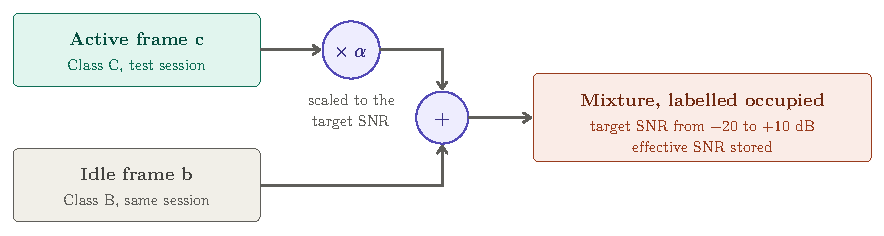
\includegraphics[width=\textwidth]{fig3-injection}
  \caption[Construction of the controlled-SNR test set]{Construction of the controlled-SNR test set. An active frame $c$ is scaled by $\alpha$ so that its estimated signal power reaches the target SNR $\gamma$ relative to the power of an idle frame $b$ from the same session, and the two are added. The effective SNR $\gamma_\mathrm{eff}$ accounts for the noise carried by $c$ (\cref{eq:m-snr-eff}).}
  \label{fig:m-injection}
\end{figure}

The mixtures are an approximation. The LTE frame already contains the receiver's noise and its 8-bit quantization, the noise added with it is environmental as well as thermal, and no fading is imposed beyond what the capture contains. The set is therefore used for controlled comparisons between detectors, while the over-the-air captures show performance under natural conditions. For hypothesis~H1, \enquote{low SNR} is defined as $\gamma \le \qty{-4}{\decibel}$ on this grid. These are the levels below the SNR wall of the energy detector for \qty{1}{\decibel} of noise uncertainty, \qty{-3.3}{\decibel} (\cref{eq:snr-wall}; \cite{tandra2008}), where an energy detector cannot be robust and a learned detector would have to show its advantage.

\section{Preprocessing}
\label{sec:m-preproc}

\emph{Frames.} Each capture is divided into non-overlapping frames of $N = \num{16384}$ complex samples, \qty{8.533}{\milli\second} at \qty{1.92}{MS/s} (\cref{fig:m-frame}). The PSS and SSS recur every \qty{5}{\milli\second} (\cref{sec:lte-sync}), so every frame of a C\textsubscript{centre} capture contains at least one complete pair. The mean of each frame's complex samples is subtracted to remove the receiver's direct-current offset \parencite{calvopalomino2015}. Every detector, classical or learned, receives the same DC-removed frames.

\emph{Spectrogram.} For the learned detectors and PCA, each frame is converted to a spectrogram (\cref{eq:stft-discrete}) with a 128-point FFT, a periodic Hann window of 128 samples and a hop of 128 samples, giving 128 frequency bins of \qty{15}{\kilo\hertz} by 128 time columns of \qty{66.7}{\micro\second}. One column is close to one OFDM symbol. The Hann window is chosen to reduce the spectral leakage from strong signals into neighbouring bins \parencite{harris1978}; the window length follows from the subcarrier spacing. Power is expressed in decibels, $S = 10 \log_{10}(\lvert X \rvert^2 + 10^{-12})$, and the bins are arranged so that frequency increases upwards when the spectrogram is drawn as an image.

\emph{Normalization.} The spectrograms are standardized with a single mean and standard deviation computed over all training frames of the current cross-validation fold, $x = (S - \mu)/s$. The same two numbers are applied unchanged to the validation and test frames, and no clipping or rescaling is applied to test data. The normalization therefore does not adapt to a changed noise floor; that is deliberate, because it is part of what H2 tests. \Cref{tab:m-preproc} lists the settings.

\begin{figure}[tbp]
  \centering
  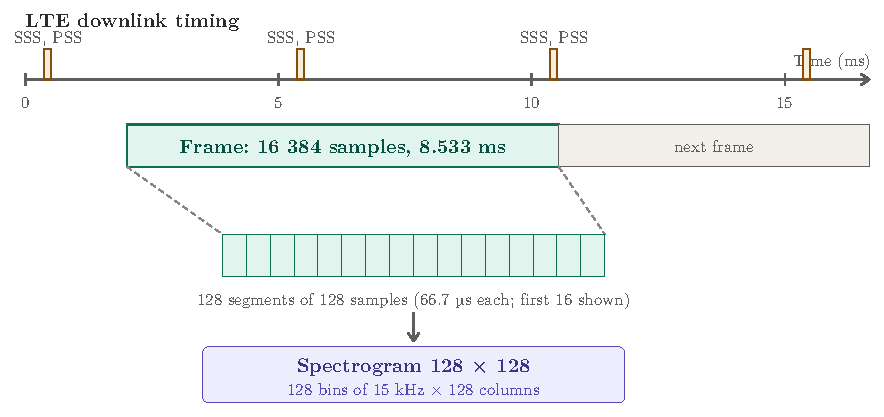
\includegraphics[width=\textwidth]{fig3-frame}
  \caption[Frame and spectrogram geometry]{Frame and spectrogram geometry. A frame of \num{16384} samples (\qty{8.533}{\milli\second}) is longer than the \qty{5}{\milli\second} period of the synchronization signals, so it always contains at least one PSS and SSS when the window covers the carrier centre. It is cut into 128 segments of 128 samples, each giving one spectrogram column of 128 bins of \qty{15}{\kilo\hertz}. Timing from \textcite[clauses~4.1, 6.11 and~6.12]{3gpp2026a}.}
  \label{fig:m-frame}
\end{figure}

\begin{table}[tbp]
  \centering
  \caption[Preprocessing settings]{Preprocessing settings.}
  \label{tab:m-preproc}
  \begin{tabularx}{\textwidth}{@{} l >{\raggedright\arraybackslash}X @{}}
    \toprule
    Setting & Value \\
    \midrule
    Sample rate & \qty{1.92}{MS/s} \\
    Frame length & \num{16384} samples (\qty{8.533}{\milli\second}), no overlap \\
    DC removal & Frame mean subtracted \\
    FFT size and window & 128 points, periodic Hann \\
    Hop & 128 samples (no overlap) \\
    Spectrogram size & $128 \times 128$ (frequency $\times$ time) \\
    Bin spacing; column duration & \qty{15}{\kilo\hertz}; \qty{66.7}{\micro\second} \\
    Scaling & $10\log_{10}$ power, then $(S-\mu)/s$ with training-fold $\mu$, $s$ \\
    \bottomrule
  \end{tabularx}
\end{table}

\section{Data Splits}
\label{sec:m-splits}

The data are split by session with four-fold cross-validation (\cref{fig:m-folds}). The sessions are divided into four groups of (at least) three. In each fold, one group is the test set, two sessions from the next group are the validation set, and the remaining sessions are the training set. Every session is therefore tested exactly once, always by models that have never seen it, and no frame from a test session is used for training, validation or normalization.

\begin{itemize}
  \item \emph{Training data:} Class~B frames at gain $g_1$ from the training sessions.
  \item \emph{Validation data:} Class~B frames at $g_1$ from the validation sessions. They are used for early stopping and for calibrating every threshold.
  \item \emph{Test data:} Class~B, C\textsubscript{centre} and C\textsubscript{offset} frames at $g_1$ from the test sessions, the controlled-SNR mixtures built from them, and, for the gain-change test, their captures at $g_2$.
\end{itemize}

With twelve sessions of \Prov{\qty{30}{\second}} captures, a fold has seven training sessions (about \num{24600} training frames), two validation sessions (about \num{7000} frames) and three test sessions.

\begin{figure}[tbp]
  \centering
  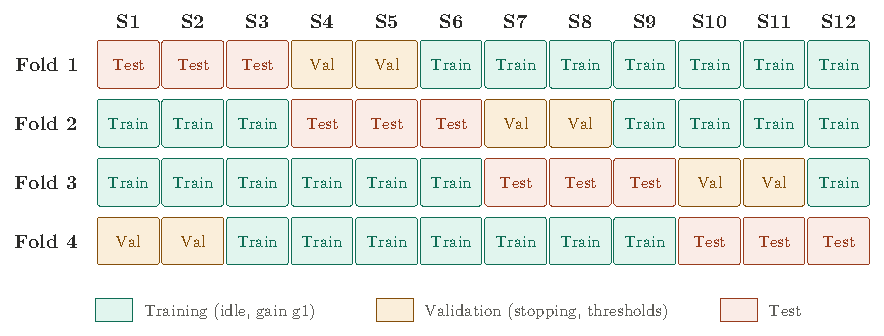
\includegraphics[width=\textwidth]{fig3-folds}
  \caption[Session-level cross-validation]{Session-level four-fold cross-validation with twelve sessions. In each fold, one group of three sessions is tested, two sessions of the next group are used for validation (early stopping and thresholds), and the rest are used for training. Every session is tested once.}
  \label{fig:m-folds}
\end{figure}

\section{Detectors}
\label{sec:m-detectors}

Seven detectors are compared (\cref{tab:m-detectors}). Four are learned from idle data: the three AI-based detectors, which are autoencoders (\cref{sec:ae}), and PCA, their linear counterpart. Of the other three, two are classical energy detectors and one exploits the known LTE synchronization signals. Each produces a score per frame, in which a larger value means that the frame is more likely to be occupied.

\begin{table}[tbp]
  \centering
  \small
  \caption[Detectors compared]{Detectors compared. All receive the same frames and are thresholded on the same idle validation data (\cref{sec:m-thresholds}).}
  \label{tab:m-detectors}
  \begin{tabularx}{\textwidth}{@{} >{\raggedright\arraybackslash}p{3.0cm} >{\raggedright\arraybackslash}X >{\raggedright\arraybackslash}X >{\raggedright\arraybackslash}X @{}}
    \toprule
    Detector & Input & Learned from & Score \\
    \midrule
    Convolutional autoencoder (primary) & Spectrogram & Idle training frames & Reconstruction MSE \\
    Fully connected autoencoder & Flattened spectrogram & Idle training frames & Reconstruction MSE \\
    Convolutional VAE & Spectrogram & Idle training frames & MSE; percentile score \parencite{tian2022} \\
    PCA & Flattened spectrogram & Idle training frames & Reconstruction MSE \\
    Fixed-threshold energy detector & DC-removed frame & Nothing (threshold only) & Average power $T$ \\
    Adaptive-threshold energy detector & DC-removed frame & Running noise estimate & $T$ divided by the noise estimate \\
    Synchronization\babelhyphen{hard}signal correlator & DC-removed frame & Nothing (threshold only) & Peak normalized correlation with the PSS \\
    \bottomrule
  \end{tabularx}
\end{table}

\subsection{Convolutional Autoencoder}
\label{sec:m-convae}

The primary detector is a convolutional autoencoder that takes the $128 \times 128$ spectrogram as a one-channel image (\cref{fig:m-convae}). Its encoder has three stages, each a $3 \times 3$ convolution followed by batch normalization and a rectified linear unit, with $2 \times 2$ max-pooling between stages and after the last. The stages have 16, 32 and 64 channels, as in the author's original model. A $1 \times 1$ convolution then reduces the 64 channels to \Prov{8}, so the code has \Prov{$8 \times 16 \times 16 = 2048$} values, an eighth of the input. The autoencoder is therefore undercomplete and must capture the most salient structure of idle spectrograms \parencite{goodfellow2016}. The decoder first maps the code back to 64 channels with a $1 \times 1$ convolution, then mirrors the encoder with bilinear $2 \times$ upsampling and $3 \times 3$ convolutions, and its output layer is linear. The network has \Prov{\num{47849}} trainable parameters. The anomaly score is the mean squared reconstruction error over the $D = \num{16384}$ elements of the spectrogram (\cref{sec:ae-pca}). The choice of a convolutional architecture follows the argument of \cref{sec:ae-architectures}; whether it is better than a fully connected one is tested, not assumed (RQ5).

\begin{figure}[tbp]
  \centering
  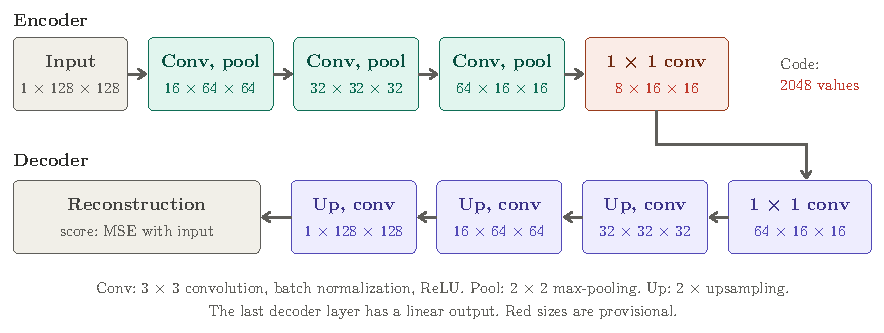
\includegraphics[width=\textwidth]{fig3-convae}
  \caption[Convolutional autoencoder]{The convolutional autoencoder, with tensor sizes (channels $\times$ frequency $\times$ time). Red sizes are provisional and may be tuned on validation data (latent channels 4, 8 or 16).}
  \label{fig:m-convae}
\end{figure}

\subsection{Fully Connected Autoencoder}
\label{sec:m-fcae}

The comparison model flattens the spectrogram to a vector of \num{16384} elements and passes it through dense layers of \Prov{256} and \Prov{128} units to the code, and back through \Prov{256} units to \num{16384} outputs, with rectified linear units between layers and a linear output. It has \Prov{\num{8471168}} trainable parameters, about 177 times as many as the convolutional autoencoder, almost all of them in its first and last layers. It is trained on the same data, with the same loss, optimizer and stopping rule as the convolutional model. Its code size is varied in an ablation (\Prov{32, 128 and 512}).

\subsection{Variational Autoencoder and Percentile Score}
\label{sec:m-vae}

The VAE uses the convolutional encoder and decoder of \cref{sec:m-convae}, with the encoder producing the mean and log-variance of a Gaussian code of \Prov{$8 \times 16 \times 16$} values \parencite{kingma2014}. It is trained to minimize the mean squared reconstruction error plus the Kullback--Leibler divergence of the code from a standard normal distribution, with weight \Prov{1}; at scoring time the code mean is decoded. Two scores are computed from the same reconstruction: the MSE, and the percentile score of \textcite{tian2022}, which combines high percentiles of the pixel-level errors in the background and signal regions of the spectrogram (\cref{sec:ae-vae}). The percentile score uses Tian et al.'s settings: a $3 \times 3$ kernel for the max- and min-pooling, a background weight of 2, a step threshold of 0.05 and the 90th and 99th percentiles (p.~4). Their description leaves two details open, which are fixed here as follows. The background mask is computed from a copy of the frame scaled to the range 0 to 1, and each percentile is taken over the pixels of its region only.

\subsection{PCA Detector}
\label{sec:m-pca}

The linear baseline projects the flattened, standardized spectrogram onto its leading principal components, computed from the training frames of the fold, and scores the frame by its mean squared reconstruction error \parencite{ruff2021}. The number of components is the smallest that explains at least \Prov{\pct{95}} of the training variance, capped at \Prov{256}. PCA is the linear counterpart of the autoencoder (\cref{sec:ae-pca}), so comparing them shows whether the non-linear model adds anything (RQ2).

\subsection{Energy Detectors}
\label{sec:m-ed}

Both energy detectors compute the average power of the DC-removed frame, $T = \frac{1}{N}\sum_{n=0}^{N-1} \lvert y(n) \rvert^2$ (\cref{eq:ed-statistic}), over all \num{16384} samples. They differ only in how their thresholds follow the noise power, the weakness identified in \cref{sec:ed}.

\begin{itemize}
  \item \emph{Fixed threshold.} The threshold on $T$ is calibrated once on the idle validation frames (\cref{sec:m-thresholds}) and never changes. This is equivalent to freezing the noise estimate at its validation value. It is the comparator for H2.
  \item \emph{Adaptive threshold.} A running noise estimate $\hat{\sigma}^2$ is kept as the median of $T$ over the most recent \Prov{$M = 64$} frames declared idle (about \qty{0.55}{\second}), initialized to the median of the validation frames. A frame is declared occupied if $T/\hat{\sigma}^2 > \kappa$. This is the constant-false-alarm-rate principle of estimating the noise level and setting the threshold relative to it \parencite[p.~121]{yucek2009}. The constant $\kappa$ is calibrated by running the same procedure over the validation stream. Each test session is processed as a stream in capture order (B, then C\textsubscript{centre}, then C\textsubscript{offset}), so the estimate can adapt to a session's noise floor before the active captures begin. An estimate is updated only by frames declared idle, so a long run of occupied frames leaves it unchanged. Because the updates depend on the decisions, the procedure is run separately for each target $\Pfa$. Mixtures of the controlled-SNR set are scored against the estimate held just before their idle frame, and Class~A captures form a stream of their own.
\end{itemize}

Under the Gaussian model of \cref{sec:ed}, the fixed threshold for a target $\Pfa$ could also be computed from the chi-square distribution of $T$ (\cref{eq:ed-threshold}). The empirical calibration is used instead, so that the energy detectors are calibrated exactly like the learned detectors. The theoretical threshold is reported for comparison.

\subsection{Synchronization-Signal Correlator}
\label{sec:m-pss}

The waveform-based detector (\cref{sec:waveform}) correlates each frame with the three possible PSS. For each root index $u \in \{25, 29, 34\}$ \parencite[Table~6.11.1.1-1]{3gpp2026a}, the length-62 Zadoff--Chu sequence $d_u(n)$ \parencite[clause~6.11.1.1]{3gpp2026a} is mapped to the subcarriers on either side of the unused DC subcarrier, $n = 0, \dots, 30$ to subcarriers $-31$ to $-1$ and $n = 31, \dots, 61$ to $+1$ to $+31$ \parencite[clause~6.11.1.2]{3gpp2026a}. A 128-point inverse FFT then gives the template $p_u(m)$, $m = 0, \dots, 127$, at the sample rate of the receiver. The score is the largest normalized correlation over the three templates and all lags $k$ at which the template lies wholly inside the frame:
\begin{equation}
  \Lambda_{\mathrm{PSS}} = \max_{u,\,k} \frac{\left\lvert \sum_{m} y(k+m)\, p_u^{*}(m) \right\rvert^2}{\sum_{m} \lvert y(k+m) \rvert^2 \, \sum_{m} \lvert p_u(m) \rvert^2},
  \label{eq:m-pss}
\end{equation}
which lies between 0 and 1 and does not depend on the receiver gain. With a frequency tolerance of \qty{1}{ppm} \parencite{rtlsdrblog2024}, the frequency error at the candidate bands is below about \qty{1}{\kilo\hertz}, a small fraction of the \qty{15}{\kilo\hertz} subcarrier spacing, so no frequency search is made. The correlator can only detect a carrier whose centre lies in the window: it is expected to work on C\textsubscript{centre} frames and to fail on C\textsubscript{offset} frames, and both results are reported. It tests only for the presence of the known sequences and decodes nothing.

\subsection{Training}
\label{sec:m-training}

The neural networks are trained with the Adam optimizer \parencite{kingma2015} (\cref{tab:m-training}). Training stops when the loss on the idle validation frames has not improved for \Prov{15} epochs, and the weights with the lowest validation loss are kept. Each model is trained with five seeds (0 to 4) in every fold, so that the variability due to initialization and batch order can be reported. Ablations of the code size use \Prov{three} seeds. The settings of \cref{tab:m-training} start from the author's original configuration, and any change made during development is based on training and validation data only.

Training runs on a GPU in Google Colab, a hosted notebook service, because training every network, fold and seed on the laptop's CPU would take weeks. The PCA detector needs no GPU and is fitted on the laptop. Only the data that training needs leave the laptop: the preprocessed Class~B spectrograms at $g_1$ of all sessions, the fold definitions, and the normalization statistics of each fold, computed on the laptop. Raw captures, active captures, captures at $g_2$, the controlled-SNR sets and all scores stay on the laptop. The idle spectrograms of every session are uploaded because each session is a training or validation session in some fold, but the training of a fold reads only that fold's training and validation sessions. A checksum of every uploaded file is verified before training. Each run saves a checkpoint at the end of every epoch and resumes from it after an interruption, because hosted sessions can be disconnected. The trained models are returned to the laptop. There they are checked against the local folds, settings, code and normalization statistics, and every expected run is checked for completeness and against its checksums, before the models are calibrated, evaluated and timed. To keep runs repeatable, the deterministic options of the GPU libraries are enabled. Results on a GPU are nevertheless not guaranteed to be bit-identical between runs, because some operations, such as the backward pass of bilinear upsampling, have no deterministic GPU implementation. The seeds still fix the initial weights and the order of the training batches. The GPU type and the library versions used are recorded with every model: \TBC{GPU and versions, from the training records}.

\begin{table}[tbp]
  \centering
  \caption[Training settings]{Training settings for the neural networks. Red values are provisional.}
  \label{tab:m-training}
  \begin{tabularx}{\textwidth}{@{} l >{\raggedright\arraybackslash}X @{}}
    \toprule
    Setting & Value \\
    \midrule
    Optimizer & Adam, learning rate \Prov{$10^{-3}$} (VAE \Prov{$10^{-4}$}), weight decay \Prov{$10^{-5}$} \\
    Batch size; maximum epochs & \Prov{64}; \Prov{100} \\
    Early stopping & Validation loss, patience \Prov{15} epochs \\
    Learning-rate schedule & Halved after \Prov{7} epochs without improvement \\
    Gradient clipping & Norm \Prov{1.0} \\
    Seeds & 0--4 (five per model and fold) \\
    Hardware & Google Colab GPU (\TBC{type}); laptop CPU (4 threads) for scoring \\
    \bottomrule
  \end{tabularx}
\end{table}

\section{Thresholds and Operating Points}
\label{sec:m-thresholds}

Every detector is operated at two target false-alarm probabilities, $\Pfa = 0.01$ and $0.05$. For each fold and detector, the threshold is the empirical $(1 - \Pfa)$ quantile of the detector's scores on the idle validation frames, taken so that at most a fraction $\Pfa$ of those scores exceeds it (\cref{fig:threshold}); for the adaptive energy detector it is $\kappa$, the quantile of $T/\hat{\sigma}^2$. A frame is declared occupied when its score exceeds the threshold. Thresholds are never set or adjusted on test data. The false-alarm rate realized on the test sessions' idle frames is reported next to the target, because a threshold calibrated on some sessions holds its rate on others only if the idle data do not change. That is the question behind RQ3 and H2.

\section{Evaluation Protocol}
\label{sec:m-eval}

\subsection{Metrics}
\label{sec:m-metrics}

For each detector, fold, seed and operating point, the predictions on the test frames give the metrics of \cref{tab:m-metrics}. Frames are counted as positives if occupied (Class~C or a mixture) and as negatives if idle (Class~B). Precision and the F1 score depend on the proportion of occupied frames in the test data, which is set by the capture plan rather than by the real occupancy of the band, so they are reported with that proportion. $\Pd$ and the realized $\Pfa$ do not depend on it. The receiver operating characteristic (ROC) curve and its area are computed from the scores without a threshold. Because each fold has its own models and score scale, the pooled curves use each score's position in its fold's idle validation distribution (its empirical quantile), so that scores from different folds are comparable.

\begin{table}[tbp]
  \centering
  \caption[Evaluation metrics]{Evaluation metrics. TP, FP, TN and FN are the counts of true positives, false positives, true negatives and false negatives, with occupied frames as positives.}
  \label{tab:m-metrics}
  \begin{tabularx}{\textwidth}{@{} l >{\raggedright\arraybackslash}X @{}}
    \toprule
    Metric & Definition \\
    \midrule
    Probability of detection, $\Pd$ (recall) & $\mathrm{TP}/(\mathrm{TP}+\mathrm{FN})$ \\
    Realized false-alarm rate, $\Pfa$ & $\mathrm{FP}/(\mathrm{FP}+\mathrm{TN})$ \\
    Precision & $\mathrm{TP}/(\mathrm{TP}+\mathrm{FP})$ \\
    F1 score & $2\,\mathrm{Precision}\cdot\Pd/(\mathrm{Precision}+\Pd)$ \\
    Confusion matrix & TP, FP, TN, FN at each operating point \\
    ROC curve and AUC & $\Pd$ against $\Pfa$ over all thresholds; area under it \\
    Precision--recall curve & Precision against recall over all thresholds \\
    \bottomrule
  \end{tabularx}
\end{table}

\subsection{SNR Stratification}
\label{sec:m-strata}

On the controlled-SNR set, $\Pd$ is reported at each level of the SNR grid, using the effective SNR of \cref{eq:m-snr-eff}. On the over-the-air C captures, the natural SNR of each frame, $P_s(c)/\hat{P}_{n,C}$ from \cref{eq:m-ps}, is estimated in the same way, and $\Pd$ is reported in bins of \Prov{\qty{2}{\decibel}}. Results for C\textsubscript{centre} and C\textsubscript{offset} are kept separate throughout.

\subsection{Uncertainty}
\label{sec:m-uncertainty}

Two sources of variability are reported. Variability due to training is the mean and standard deviation of each metric over the five seeds of each neural network; PCA and the classical detectors are deterministic and have no such variability. Variability due to the data is estimated with the bootstrap, which estimates the sampling distribution of a statistic from the observed data \parencite{efron1979}. Because frames within a session are not independent, the resampling units are sessions, not frames. The test predictions of the four folds are pooled, so that every session contributes once; \num{1000} bootstrap samples are drawn by resampling sessions with replacement, the metric, averaged over the five seeds, is recomputed on the frames of each sample, and the 2.5th and 97.5th percentiles give a \pct{95} interval. Differences between two detectors are bootstrapped in the same way, with both detectors evaluated on the same resampled sessions.

\subsection{Robustness}
\label{sec:m-robustness}

RQ3 is answered with three comparisons (\cref{tab:m-robustness}). Across sessions, the pooled cross-validation results already measure performance on sessions, days and positions that the models have not seen, and they are also broken down by session, by time of day (day or night sessions, \cref{sec:m-sessions}) and, where more than one position exists, by position. Across gain settings, the models and thresholds calibrated at $g_1$ are applied to the same test sessions' captures at $g_2$. The change of gain lowers the carrier's level by about \qty{8}{\decibel} but the idle level by only about \qty{2}{\decibel}, because the receiver's own noise dominates at these gains (\cref{sec:m-capture}); both changes are measured in every session. The receiver noise floor of each session and gain is tracked with the Class~A captures, so that changes of the idle data can be attributed to the receiver or to the environment.

\begin{table}[tbp]
  \centering
  \caption[Robustness comparisons]{Robustness comparisons for RQ3 and H2.}
  \label{tab:m-robustness}
  \begin{tabularx}{\textwidth}{@{} >{\raggedright\arraybackslash}p{3.0cm} >{\raggedright\arraybackslash}X >{\raggedright\arraybackslash}X @{}}
    \toprule
    Comparison & Training and calibration & Test \\
    \midrule
    Across sessions & Training and validation sessions of each fold, $g_1$ & Unseen test sessions, $g_1$ \\
    Across gain settings & As above, $g_1$ & The same test sessions, $g_2$ \\
    Across times and positions & As above & Pooled results broken down by time of day and position \\
    \bottomrule
  \end{tabularx}
\end{table}

\subsection{Hypothesis Tests}
\label{sec:m-hypotheses}

\emph{H1.} On the controlled-SNR set at gain $g_1$ and $\gamma \le \qty{-4}{\decibel}$, the difference
\begin{equation}
  \Delta\Pd = \Pd(\text{convolutional autoencoder}) - \Pd(\text{adaptive energy detector})
  \label{eq:m-h1}
\end{equation}
is computed at each operating point, pooled over the low-SNR levels. H1 is supported at an operating point if the \pct{95} bootstrap interval of $\Delta\Pd$ lies entirely above zero, and it is not supported otherwise. The primary test pools the mixtures built from C\textsubscript{centre} and C\textsubscript{offset} captures, and each source is also reported separately.

\emph{H2.} For the gain-$g_2$ test data, with thresholds calibrated at $g_1$, the departure of each detector from its calibrated behaviour is measured in two ways. The first is the absolute difference between the realized $\Pfa$ on the idle test frames and the target $\Pfa$. The second is the absolute difference between $\Pd$ at $g_2$ and at $g_1$ on the controlled-SNR set, with the mixtures of both sources pooled, averaged over the SNR levels that have mixtures at both gains. H2 is supported at an operating point if both departures of the convolutional autoencoder are smaller than those of the fixed-threshold energy detector, with \pct{95} bootstrap intervals of the paired differences entirely on that side. The adaptive energy detector is reported alongside as the reference for how much adaptation alone recovers.

\subsection{Failure Analysis}
\label{sec:m-failures}

For each detector a sample of false alarms and missed detections is inspected: their spectrograms, session, time of day, gain and estimated SNR. The aim is to relate errors to identifiable causes such as interference in the idle window, a changed noise floor or low SNR. Any cause found is reported with the results.

\section{Computational Cost}
\label{sec:m-compute}

\ref{rq:compute} asks whether the detectors can run in real time on the laptop. The question concerns the implementation as it would be used, so the scoring code of the neural networks is optimized (\cref{sec:m-optim}), and every detector is timed exactly as it is evaluated (\cref{sec:m-timing}).

\subsection{Optimization of Scoring}
\label{sec:m-optim}

Three changes reduce the work that the neural networks do for each frame. None of them may change a score beyond floating-point rounding, because the scores are what the evaluation compares, and the same scoring code is used in the evaluation, in the timing and in the demonstration.

\begin{itemize}
  \item \emph{Batch normalization folded into the convolutions.} When a trained network scores a frame, each batch-normalization layer multiplies every channel by one constant and adds another, both fixed by the statistics and parameters stored during training. The multiplication is therefore absorbed into the kernel of the convolution before the layer, and the addition into its bias, which removes one pass over every feature map of the convolutional networks.
  \item \emph{Channels-last memory order.} The feature maps of the convolutional networks are stored with the channels of each pixel next to each other, an alternative memory order that PyTorch supports for convolutions on the CPU, instead of one complete image per channel.
  \item \emph{Percentiles of the PER score.} The two percentiles of the PER score are computed with NumPy's percentile function instead of PyTorch's quantile function. Both interpolate linearly between order statistics and give identical values.
\end{itemize}

The fully connected autoencoder and the PCA detector contain neither convolutions nor batch normalization and are unchanged. The tests of the code (\cref{tab:app-tests}) check that the optimized networks reproduce the reconstructions of the trained networks to within $10^{-5}$ of the largest reconstructed value, and that the PER scores are identical. To measure the effect of the optimization, each neural network is also timed in its original form, as trained, with the original percentile computation. The two forms are timed on the same frames, alternating frame by frame, so that both see the same state of the laptop, and the ratio of their median latencies is reported in \cref{sec:r-compute}.

\subsection{Timing}
\label{sec:m-timing}

Latency and throughput are measured on the host laptop with the library versions of \cref{tab:m-hw-sw} and PyTorch limited to four threads, one per physical core of the processor. All timings are taken with the laptop on mains power and set to its Performance power profile, so that the processor runs at full speed and the timings are comparable; the timing program refuses any other known power state. Before any timing, every detector runs in turn for \qty{5}{\second}, because start-up effects of the program were found to slow the first detector timed for several seconds, longer than its own warm-up. After \num{50} warm-up frames, each detector then scores \num{1000} frames one at a time, and the time per frame is measured with Python's high-resolution performance counter. The median and the 95th percentile are reported separately for preprocessing (DC removal, spectrogram and standardization), for scoring, and end to end. Throughput is measured in frames per second with batches of 64 frames. The real-time factor is the processing time per frame divided by the frame duration, \qty{8.533}{\milli\second}; a value below one means the detector keeps up with the receiver. The CPU model, the thread count, the library versions and the power state are recorded with each measurement.

\section{Real-Time Demonstration}
\label{sec:m-demo}

The demonstration runs the complete chain live on the laptop (\cref{fig:m-demo}). Samples are read from the receiver at \qty{1.92}{MS/s} in blocks of one frame. Each frame is preprocessed and scored by the chosen detector with its calibrated threshold. The time, centre frequency, gain, score, decision and processing time of every frame are logged, and an optional live view shows the rolling spectrogram and the occupancy decisions; it is redrawn at most four times per second, and not while frames are waiting, so that it does not slow the detector. A short buffer of 32 frames (\qty{0.27}{\second}) separates reading from processing. If processing falls behind, the oldest frames are dropped and counted, so that the decisions stay current. Samples lost before they reach the program, for example by an overflow of the USB link, are estimated from the arrival times of the blocks and reported. Like the timings, the demonstration runs on mains power with the Performance profile. A short logged run on the chosen carrier (\cref{sec:m-survey}) illustrates occupancy over time in Chapter~4.

\begin{figure}[tbp]
  \centering
  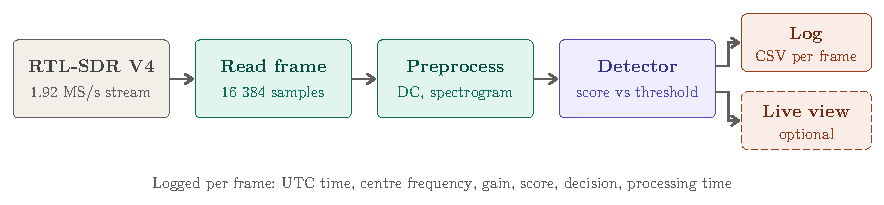
\includegraphics[width=\textwidth]{fig3-demo}
  \caption[Real-time demonstration]{Real-time demonstration. Frames are read from the receiver, preprocessed and scored as in the evaluation, and each decision is logged with its time and processing time.}
  \label{fig:m-demo}
\end{figure}

\section{Ethics, Reproducibility and Threats to Validity}
\label{sec:m-ethics}

\emph{Ethics.} Reception is passive: the study transmits nothing and measures only power and spectral structure. The \syncsignal{} correlator tests only for the presence of known sequences. The cell-search tool also decodes the MIB that each cell broadcasts, from which it reports only the carrier's bandwidth and two control-channel settings; only this mode of the tool is used, and no other system information, user data or other content is decoded or recorded.

\emph{Reproducibility.} Every result file records the configuration, the seeds, the version of the code and the library versions, and every trained model also records the device it was trained on. The code version is the Git commit together with a checksum of the source files; for the models trained on Colab, where Git is not available, it is the checksum, which must match that of the code on the laptop. The complete code is available at \url{https://github.com/jimroxodezi/masters-thesis}, and the modules that compute the reported results are listed in \cref{app:code}; the captures and labels are released if the supervisor approves.

\emph{Threats to validity.}
\begin{itemize}
  \item \emph{One receiver, one band, one city.} The results may not transfer to other receivers, bands or environments (Chapter~1). Two positions and two times of day widen the conditions but do not remove this limit. Both positions are at one home, so the transfer of a detector to another building, neighbourhood or set of base stations is not tested; the comparison between positions measures the effect of a change of direction and surroundings within one home.
  \item \emph{Labels.} Capture-level labels could be wrong if a carrier were missed in an idle window or a cell switched off during an active capture. The second labelling pass and the inspection of spectrograms reduce this risk.
  \item \emph{Idle data.} Interference in the idle windows is kept as part of the idle class. If it differs between sessions, it raises false alarms, which is a real effect rather than an artefact, but it complicates the comparison of sessions.
  \item \emph{Dynamic range.} The strong carrier limits the gain (\cref{app:gains}), so the idle data are dominated by the receiver's own noise and the environment contributes little to them. The results therefore describe detection against the noise of a low-cost receiver near a strong carrier, and the gain-change test shifts the idle level by only about \qty{2}{\decibel}.
  \item \emph{Controlled-SNR mixtures.} They approximate rather than reproduce weak signals (\cref{sec:m-injection}). The over-the-air captures complement them.
  \item \emph{Number of sessions.} With about twelve sessions the bootstrap intervals will be wide. Their width is reported rather than hidden.
  \item \emph{Tuning.} All settings are chosen on training and validation data. The test sessions are scored only after the configuration is frozen.
\end{itemize}

\section{Summary}
\label{sec:m-summary}

The method compares seven detectors on identical frames of real captures from an RTL-SDR Blog V4 sampling at \qty{1.92}{MS/s}, a rate tied to the LTE time unit. Data are captured in sessions, each with receiver noise, idle and active windows at two gain settings. Ground truth is set per capture and justified by the always-on reference signals of an active carrier. A controlled-SNR set with exact labels complements the natural captures. The learned detectors are trained only on idle frames. Every detector is calibrated on idle validation sessions at false-alarm probabilities of \pct{1} and \pct{5}, and evaluated on unseen sessions through session-level cross-validation, with uncertainty over seeds and sessions. Two hypotheses are tested with stated criteria, and the computational cost is measured on the laptop that would run the detector. Chapter~4 reports the results.
